% -*- TeX -*- -*- UK -*- -*- Soft -*-

\chapter{Google Colaboratory}
\label{sec:Google Colaboratory}

The early content of chapter is based on material from  \cite{LiuCoLab2019}.

\section{Getting Started with Colab}

Open \lstinline{https://colab.research.google.com} in a browser and click on \lstinline{NEW PYTHON 3 NOTEBOOK} in the lower right corner.  This should launch a notebook in your browser. 

Once you have a notebook created, it'll be saved in your Google Drive (Colab Notebooks folder). You can access it by visiting your Google Drive page, then either double-click on the file name, or right-click, and then choose ``Open with Colab''. 

Rename the notebook and save it. 

\section{Saving on GitHub}

Create a new repository, and commit at least one file to the master branch, so that the github repo has a master branch (not an empy repo).
In the colab File menu select save copy to github.
You will be asked to authorise the access and henceforth it should work without further authorisation.
Select the require repository and its master branch and then click on OK.
In future, the file can be opened from within GitHub by clicking on the button.

\begin{figure*}[h]
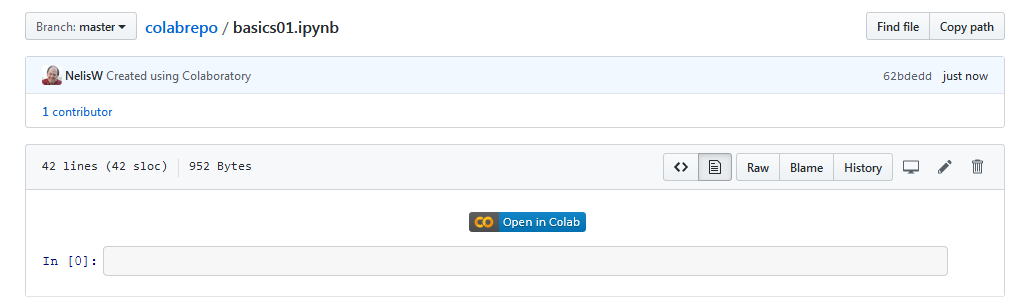
\includegraphics[width=\textwidth]{colabrepo01}
\end{figure*}


\section{Enabling GPU Support}

To turn on GPU for your Deep Learning projects, just go to the drop-down menu and select ``Runtime --- Change runtime type --- Hardware accelerator'' and choose GPU

\section{Working with the Notebook}

The colab notebooks are similar to Jupyter notebooks, use the same commands.
You can also save files to your colab folder (and presumably then also to github).

\section{Introduction to TensorFlow}

\subsection{Tensors}

TensorFlow bases its name on the word ``tensor''. What is a tensor anyway? In short, a multi-dimensional array. Let's see what that means!

\begin{itemize}
\item We have one single number, e.g. 6, we call it a ``scalar'';
\item We have three numbers, e.g. [ 6, 8, 9], we call that a ``vector'';
\item We have a table of numbers, e.g. [[6, 8, 9], [2, 5, 7]], we call that a ``matrix'' (which has two rows and three columns);
\item We have a table of table of numbers, e.g. [[[6, 8, 9], [2, 5, 7]], [[6, 8, 9], [2, 5, 7]]], and…we are running out of words here :( My friend, that is a tensor! A tensor is just a generalized form of arrays that can have any number of dimensions.
\end{itemize}

In TensorFlow jargons, a scalar is a rank 0 tensor, a vector is rank 1 and matrix rank 2 etc. There are three frequently used types of tensors: constant, variable, and placeholder which are explained below.

\subsection{Types of Tensors}

Constants are exactly what their names refer to. They are the fixed numbers in your equation. To define a constant, we can do this:

\begin{lstlisting}[language=Python]
a = tf.constant(1, name='a_var')
b = tf.constant(2, name='b_bar')
\end{lstlisting}
Aside from the value 1, we can also provide a name such as \lstinline{a_var} for the tensor which is separate from the Python variable name \lstinline{a}. It's optional but will be helpful in later operations and troubleshooting.

After defining, if we print variable a, we'll have:

\begin{lstlisting}[language=Python]
<tf.Tensor 'a_var:0' shape=() dtype=int32>
\end{lstlisting}
Variables are the model parameters to be optimized, for example, the weights and biases in your neural networks. Similarly, we can also define a variable and show its contents like this:

\begin{lstlisting}
c = tf.Variable(a + b)
c
\end{lstlisting}
and have this output:

\begin{lstlisting}
<tf.Variable 'Variable:0' shape=() dtype=int32_ref>
\end{lstlisting}
But it's important to note that all variables need to be initialized before use like this:

\begin{lstlisting}
init = tf.global_variables_initializer()
\end{lstlisting}
You might have noticed that the values of a and b, i.e., integers 1 and 2 are not showing up anywhere, why?

That's an important characteristic of TensorFlow --- ``lazy execution'', meaning things are defined first, but not run. It's only executed when we tell it to do, which is done through the running of a session! (Note that TensorFlow also has eager execution. Check here for more info)

\subsection{Session and Computational Graph}

Now let's define a session and run it:

\begin{lstlisting}
with tf.Session() as session:                    
    session.run(init)                            
    print(session.run(c))
\end{lstlisting}
Notice that within the session we run both the initialization of variables and the calculation of c. We defined c as the sum of a and b:

\begin{lstlisting}
c = tf.Variable(a + b)
\end{lstlisting}
This, in TensorFlow and Deep Learning speak, is the ``computational graph''. Sounds pretty sophisticated, right? But it's really just an expression of the calculation we want to carry out!

\subsection{Placeholder}

Another important tensor type is the placeholder. Its use case is to hold the place for data to be supplied. For example, we defined a computational graph, and we have lots of training data, we can then use placeholders to indicate we'll feed these in later.

Let's see an example. Say we have an equation like this:

\begin{equation}
y = ax^2+bbx+c
\end{equation}

Instead of one single x input, we have a vector of x's. So we can use a placeholder to define x:

\begin{lstlisting}
x = tf.placeholder(dtype=tf.float32)
\end{lstlisting}
We also need the coefficients. Let's use constants:

\begin{lstlisting}
a = tf.constant(1, dtype=tf.float32)
b = tf.constant(-20, dtype=tf.float32)
c = tf.constant(-100, dtype=tf.float32)
\end{lstlisting}
Now let's make the computational graph and provide the input values for x:

\begin{lstlisting}
y = a * (x ** 2) + b * x + c
x_feed = np.linspace(-10, 30, num=10)
\end{lstlisting}
And finally, we can run it:

\begin{lstlisting}
with tf.Session() as sess:
  results = sess.run(y, feed_dict={x: x_feed})
print(results)
\end{lstlisting}
which gives us:

\begin{lstlisting}
[ 200.         41.975304  -76.54321  -155.55554  -195.06174  -195.06174  -155.55554   -76.54324    41.97534   200.      ]
\end{lstlisting}
\subsection{Putting it All Together}

Now that we have the basics of TensorFlow, let's do a mini project to build a linear regression model, aka, a neural network :) (The code is adapted from the example given in TensorFlow's guide here)

Let's say we have a bunch of x, y value pairs, and we need to find the best fit line. First, since both x and y have values to be fed in the model, we'll define them as placeholders:

\begin{lstlisting}
x = tf.placeholder(dtype=tf.float32, shape=(None, 1))
y_true = tf.placeholder(dtype=tf.float32, shape=(None, 1))
\end{lstlisting}
The number of rows is defined as None to have the flexibility of feeding in any number of rows we want.

Next, we need to define a model. In this case here, our model has just one layer with one weight and one bias.

\begin{marginfigure}
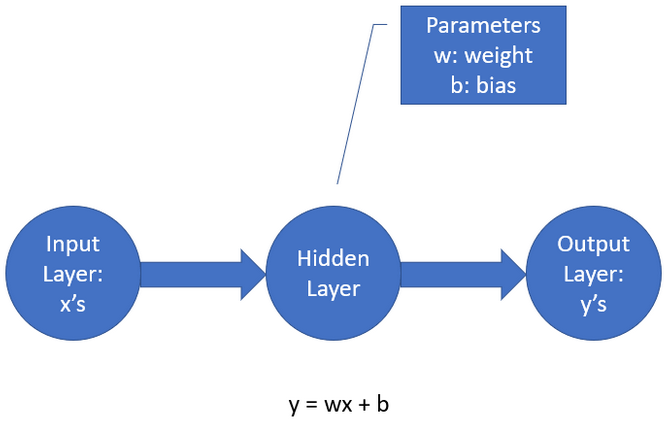
\includegraphics{colabrepo03}
\end{marginfigure}


TensorFlow allows us to define neural network layers very easily:

\begin{lstlisting}
linear_model = tf.layers.Dense(
                   units=1, 
                   bias_initializer=tf.constant_initializer(1))
y_pred = linear_model(x)
\end{lstlisting}
The number of units is set to be one since we only have one node in the hidden layer.

Furthermore, we need to have a loss function and set up the optimization method. The loss function is basically a way to measure how bad our model is when measured using the training data, so of course, we want it to be minimized. We'll use the gradient descent algorithm to optimize this loss function (I'll explain gradient descent in a future post).

\begin{lstlisting}
optimizer = tf.train.GradientDescentOptimizer(0.01)
train = optimizer.minimize(loss)
\end{lstlisting}
Then we can initialize all the variables. In this case here, all our variables including weight and bias are part of the layer we defined above.

\begin{lstlisting}
init = tf.global_variables_initializer()
\end{lstlisting}
Lastly, we can supply the training data for the placeholders and start the training:

\begin{lstlisting}
x_values = np.array([[1], [2], [3], [4]])
y_values = np.array([[0], [-1], [-2], [-3]])

with tf.Session() as sess:
  sess.run(init)
  for i in range(1000):
    _, loss_value = sess.run((train, loss),
                             feed_dict={x: x_values, y_true: y_values})
\end{lstlisting}
and we can get the weights and make the predictions like so:

\begin{lstlisting}
weights = sess.run(linear_model.weights)
bias = sess.run(linear_model.bias)
preds = sess.run(y_pred, 
                 feed_dict={x: x_values})
\end{lstlisting}
which yields these predictions:

\begin{lstlisting}
[[-0.00847495]  [-1.0041066 ]  [-1.9997383 ]  [-2.99537   ]]
\end{lstlisting}
If you are curious like me, you can verify to confirm the model did make the predictions using its trained weight and bias by:

\begin{lstlisting}
w = weights[0].tolist()[0][0]
b = weights[1].tolist()[0]
x_values * w + b
\end{lstlisting}
which gives us exactly the same result!

\begin{lstlisting}
array([[-0.00847495],        [-1.00410664],        [-1.99973834],        [-2.99537003]])
\end{lstlisting}
Voila! A simple neural network built using TensorFlow in Google Colab! Hope you find this tutorial interesting and informative.

\subsection{Final thoughts}

Cloud computing is definitely the future of Deep Learning computing. Google Colab is clearly a future-ready product. It's hard to imagine people still wanting to spend time setting up Deep Learning environments when we can just fire up a notebook on the cloud and start building models!


